\FloatBarrier
\subsection{Dự báo SOH, dung lượng và RUL: HiGBDT và HiPINN}\label{sec:e33res}

\Cref{tab:e33} cho MAE của SOH dự báo ở hai ngân sách nhãn, 30\,\% nhãn hoặc mọi cell huấn luyện. Lịch sử SOH của cell kiểm tra tới gốc là dung lượng đo. Hai mô hình chỉ dựa vào chính cell là giữ nguyên và ngoại suy tuyến tính có sai số gấp 1{,}8--10{,}3 lần HiPINN nên không đưa vào bảng (có trong \Cref{fig:e33mae}).

\begin{table}[!htbp]\centering\small
\caption[MAE của SOH dự báo theo mô hình]{MAE theo cell ($\times10^{-3}$) của SOH dự báo trên mọi chu kỳ đo được sau gốc ($0{,}2L$, $0{,}4L$, $0{,}6L$), trung bình qua 3 lần lặp; in đậm là thấp nhất mỗi hàng. $^{*}$/$^{\dagger}$: HiPINN tốt hơn/kém hơn có ý nghĩa thống kê so với HiGBDT theo kiểm định Wilcoxon ghép cặp theo cell (Holm qua bốn bộ, $p<0{,}05$).}\label{tab:e33}
\begin{adjustbox}{max width=\textwidth}\begin{tabular}{lrrrrrrrr}\toprule
 & \multicolumn{8}{c}{MAE của SOH dự báo ($\times10^{-3}$) $\downarrow$} \\\cmidrule(lr){2-9}
 & \multicolumn{3}{c}{chỉ đặc trưng gốc} & \multicolumn{5}{c}{có đặc trưng lịch sử} \\\cmidrule(lr){2-4}\cmidrule(lr){5-9}
Bộ & \begin{tabular}[b]{@{}r@{}}GBDT\\theo tầm\end{tabular} & \begin{tabular}[b]{@{}r@{}}PINN-\\dự báo\end{tabular} & \begin{tabular}[b]{@{}r@{}}PINN-\\GBDT\end{tabular} & \begin{tabular}[b]{@{}r@{}}\\HiGBDT\end{tabular} & \begin{tabular}[b]{@{}r@{}}PINN có\\lịch sử\end{tabular} & \begin{tabular}[b]{@{}r@{}}Theo\\đời\end{tabular} & \begin{tabular}[b]{@{}r@{}}\\HiPINN-w\end{tabular} & \begin{tabular}[b]{@{}r@{}}\\HiPINN\end{tabular} \\\midrule
\multicolumn{9}{@{}l}{\textit{30\,\% nhãn}} \\
XJTU & 18{,}71 & 31{,}23 & 26{,}51 & 17{,}34 & 27{,}25 & 19{,}54 & 25{,}26 & \textbf{16{,}37}\phantom{$^{*}$} \\
TJU & 7{,}55 & 9{,}66 & 9{,}01 & 7{,}07 & 9{,}03 & 8{,}91 & 8{,}05 & \textbf{6{,}10}$^{*}$ \\
MIT & 12{,}07 & 16{,}72 & 14{,}47 & \textbf{10{,}24} & 18{,}27 & 12{,}72 & 12{,}00 & 10{,}29\phantom{$^{*}$} \\
HUST & 14{,}13 & 18{,}88 & 15{,}82 & 12{,}78 & 16{,}41 & 12{,}84 & 13{,}90 & \textbf{12{,}27}$^{*}$ \\
\addlinespace[3pt]
\multicolumn{9}{@{}l}{\textit{mọi cell huấn luyện}} \\
XJTU & 15{,}81 & 15{,}15 & 14{,}49 & 13{,}97 & 16{,}79 & 15{,}59 & 15{,}42 & \textbf{13{,}21}$^{*}$ \\
TJU & 6{,}30 & 7{,}44 & 6{,}99 & 5{,}89 & 7{,}08 & 7{,}00 & 6{,}84 & \textbf{5{,}09}$^{*}$ \\
MIT & 10{,}82 & 13{,}15 & 11{,}66 & 9{,}43 & 13{,}78 & 11{,}20 & 9{,}93 & \textbf{9{,}27}$^{*}$ \\
HUST & 12{,}17 & 13{,}61 & 11{,}79 & 11{,}24 & 12{,}54 & 11{,}24 & 10{,}90 & \textbf{10{,}35}$^{*}$ \\
\bottomrule\end{tabular}\end{adjustbox}\end{table}

Trước hết, xét tác động của việc thêm lịch sử vào từng nhánh. Với GBDT, đặc trưng lịch sử giúp rõ rệt: HiGBDT có MAE bằng 0{,}85--0{,}94 lần GBDT theo tầm, thấp hơn có ý nghĩa thống kê ở cả hai ngân sách trên cả bốn bộ. Cây quyết định dùng được trực tiếp những thông tin như độ dốc trên nhiều cửa sổ hay mức dao động gần đây để nhận ra cell đang suy giảm nhanh hay chậm. Với PINN-dự báo, lợi ích không đều: bản có lịch sử có MAE bằng 0{,}87--1{,}11 lần bản không có lịch sử, thấp hơn có ý nghĩa thống kê ở cả hai ngân sách trên HUST. Một cách giải thích: mạng chỉ chọn hai tham số $(a, \lambda)$ của một đường suy giảm có dạng cố định, nên thông tin thêm từ lịch sử chủ yếu giúp ước lượng tốc độ hiện tại, điều mà hai độ dốc trong $\mathbf{z}_k$ đã có một phần, trong khi số đầu vào tăng hơn gấp đôi. Vì vậy HiPINN giữ PINN-dự báo không có lịch sử làm nhánh PINN, còn lịch sử được đưa vào mô hình qua hai nhánh kia.

HiPINN-w, phương án đầu của HiPINN, chọn trọng số của ba nhánh và nhánh PINN trên nửa tập xác thực dùng để chọn. Nửa này chỉ có 3--7 cell mỗi lượt. Trên chính nửa đó (\Cref{tab:e33val}), HiPINN-w có MAE bằng 0{,}71--0{,}92 lần HiGBDT. Trên nửa hiệu chỉnh, tỉ số này là 0{,}80--1{,}45, và trên cell kiểm tra là 0{,}97--1{,}46, cao hơn HiGBDT ở 7/8 trường hợp. Trọng số chọn trên vài cell phản ánh chính các cell đó nhiều hơn là quy luật chung, nên ưu thế mất đi khi chuyển sang cell khác. HiPINN vì vậy dùng trung vị, không có trọng số cần chọn (\Cref{sec:e33pp}).

Xét tiếp HiPINN, mô hình lấy trung vị của ba nhánh. HiPINN có MAE thấp nhất trong tám mô hình của \Cref{tab:e33} ở 7/8 trường hợp (bộ $\times$ ngân sách). So với HiGBDT, nhánh tốt nhất khi đứng riêng, MAE của HiPINN bằng 0{,}86--1{,}01 lần và thấp hơn ở 7/8 trường hợp. Theo kiểm định ghép cặp, HiPINN tốt hơn có ý nghĩa thống kê ở 6/8 và kém hơn có ý nghĩa thống kê ở 0/8 trường hợp, với 62--82\,\% số cell có sai số thấp hơn. So với PINN-GBDT, MAE của HiPINN bằng 0{,}62--0{,}91 lần (thấp hơn có ý nghĩa thống kê ở 8/8 trường hợp). Trung vị cũng tốt hơn hai cách ghép còn lại: MAE của HiPINN bằng 0{,}65--0{,}95 lần HiPINN-w (thấp hơn ở 8/8 trường hợp) và 0{,}79--0{,}99 lần HiPINN-tb, tức trung bình đều ba nhánh (thấp hơn ở 8/8). Khi một nhánh sai xa, trung bình bị kéo theo, còn trung vị đi theo hai nhánh còn lại.

Dạng trung vị được chọn sau khi đã thấy kết quả kiểm tra của HiPINN-w, nên cần một kiểm tra không dùng cell kiểm tra. Nửa hiệu chỉnh không dùng để chọn gì cho các mô hình HiGBDT, HiPINN-w, HiPINN-tb và HiPINN, và sai số của trung vị trên nửa này chưa được xem khi quyết định. Trên nửa này (\Cref{tab:e33val}), HiPINN có MAE thấp hơn HiPINN-w ở 7/8 trường hợp. So với HiGBDT, HiPINN thấp hơn ở 4/4 bộ khi học trên mọi cell huấn luyện (tốt hơn có ý nghĩa thống kê ở 3) và 2/4 bộ với 30\,\% nhãn. Kết quả cùng chiều với tập kiểm tra khi học trên mọi cell huấn luyện. Với 30\,\% nhãn, ưu thế của HiPINN so với HiGBDT trên tập kiểm tra chưa được nửa hiệu chỉnh xác nhận, nên một phần ưu thế đó có thể do chính việc chọn dạng trung vị sau khi xem kết quả.

\begin{table}[!htbp]\centering\small
\caption[MAE của SOH dự báo trên hai nửa tập xác thực]{MAE theo cell ($\times10^{-3}$) của SOH dự báo trên hai nửa tập xác thực; mỗi cell lấy trung bình qua các lượt mà nó thuộc nửa đó. Nửa chọn là nơi chọn trọng số của HiPINN-w; nửa hiệu chỉnh không dùng để chọn gì cho các mô hình trong bảng. In đậm là thấp nhất trong mỗi nửa. $^{*}$/$^{\dagger}$: trên nửa hiệu chỉnh, HiPINN tốt hơn/kém hơn có ý nghĩa thống kê so với HiGBDT (Wilcoxon ghép cặp theo cell, Holm qua bốn bộ, $p<0{,}05$).}\label{tab:e33val}
\begin{adjustbox}{max width=\textwidth}\begin{tabular}{lrrrrrrr}\toprule
 & \multicolumn{7}{c}{MAE theo cell ($\times10^{-3}$) $\downarrow$} \\\cmidrule(lr){2-8}
 & \multicolumn{3}{c}{nửa chọn} & \multicolumn{4}{c}{nửa hiệu chỉnh} \\\cmidrule(lr){2-4}\cmidrule(lr){5-8}
Bộ & \begin{tabular}[b]{@{}r@{}}\\HiGBDT\end{tabular} & \begin{tabular}[b]{@{}r@{}}\\HiPINN-w\end{tabular} & \begin{tabular}[b]{@{}r@{}}\\HiPINN\end{tabular} & \begin{tabular}[b]{@{}r@{}}\\HiGBDT\end{tabular} & \begin{tabular}[b]{@{}r@{}}\\HiPINN-w\end{tabular} & \begin{tabular}[b]{@{}r@{}}\\HiPINN-tb\end{tabular} & \begin{tabular}[b]{@{}r@{}}\\HiPINN\end{tabular} \\\midrule
\multicolumn{8}{@{}l}{\textit{30\,\% nhãn}} \\
XJTU & 13{,}07 & \textbf{10{,}64} & 12{,}49 & \textbf{16{,}56} & 23{,}94 & 18{,}70 & 16{,}79\phantom{$^{*}$} \\
TJU & 6{,}95 & \textbf{5{,}53} & 6{,}18 & 6{,}61 & \textbf{5{,}29} & 6{,}55 & 5{,}79\phantom{$^{*}$} \\
MIT & 8{,}88 & \textbf{8{,}19} & 8{,}71 & \textbf{9{,}93} & 12{,}45 & 11{,}86 & 10{,}39\phantom{$^{*}$} \\
HUST & 11{,}35 & \textbf{10{,}03} & 11{,}45 & 12{,}30 & 13{,}06 & 13{,}18 & \textbf{12{,}26}\phantom{$^{*}$} \\
\addlinespace[3pt]
\multicolumn{8}{@{}l}{\textit{mọi cell huấn luyện}} \\
XJTU & 12{,}37 & \textbf{10{,}15} & 11{,}46 & 13{,}77 & 15{,}95 & 13{,}23 & \textbf{12{,}91}$^{*}$ \\
TJU & 6{,}36 & \textbf{4{,}51} & 5{,}35 & 6{,}06 & 5{,}18 & 5{,}35 & \textbf{5{,}07}$^{*}$ \\
MIT & 8{,}26 & \textbf{7{,}58} & 8{,}08 & 9{,}09 & 9{,}98 & 10{,}59 & \textbf{8{,}87}\phantom{$^{*}$} \\
HUST & 10{,}54 & \textbf{8{,}67} & 9{,}80 & 11{,}53 & 11{,}22 & 10{,}89 & \textbf{10{,}75}$^{*}$ \\
\bottomrule\end{tabular}\end{adjustbox}\end{table}

\begin{figure}[!htbp]\centering
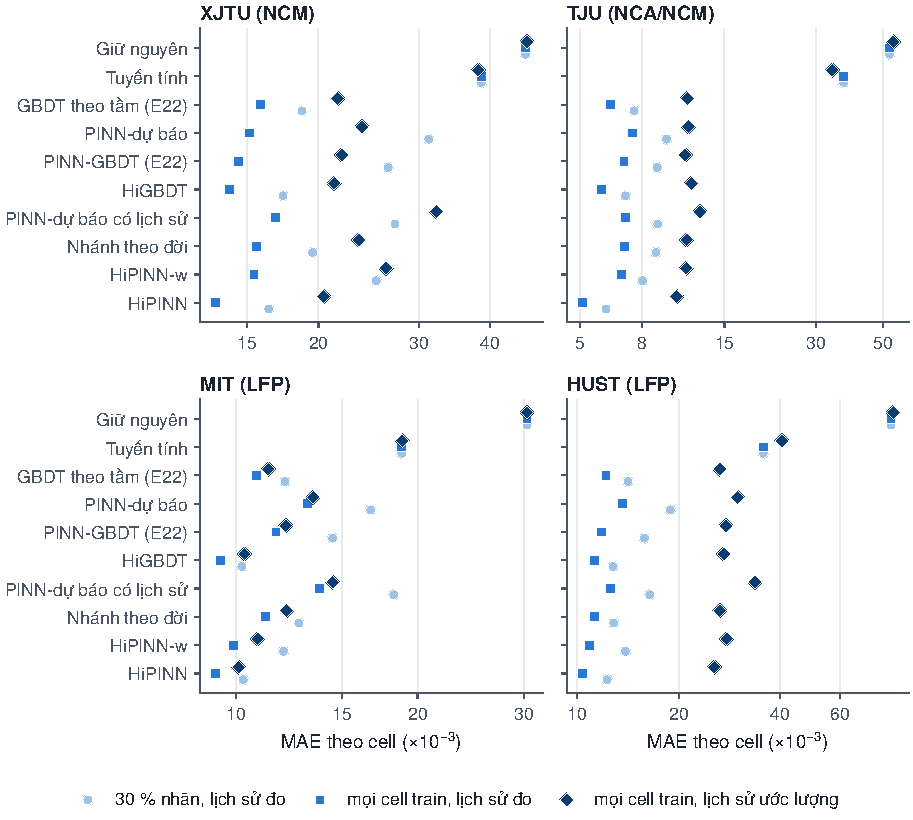
\includegraphics[width=\textwidth]{graphics/fig_e33_mae.pdf}
\caption[MAE của SOH dự báo theo mô hình và ngân sách nhãn]{MAE theo cell (trung bình qua 3 lần lặp, thang log) của các mô hình ở hai ngân sách nhãn, 30\,\% nhãn hoặc mọi cell huấn luyện; lịch sử SOH tới gốc là dung lượng đo.}\label{fig:e33mae}
\end{figure}

Sai số dự báo không đều theo tuổi của cell. \Cref{fig:e33tail} chia sai số theo phần đời của chính cell (mọi cell huấn luyện, lịch sử đo). Sai số của các mô hình nhìn chung tăng về cuối đời, và với HiPINN lớn nhất ở 10\,\% đời cuối trên cả bốn bộ. Ở MIT, MAE trên 10\,\% đời cuối là 26{,}2 với PINN-GBDT và 20{,}6 với HiPINN, giảm 22\,\% ($\times10^{-3}$; HiGBDT 20{,}8). Phần sai số còn lại chủ yếu là dự báo cao hơn thực tế: độ lệch trung bình ở đoạn này là +12{,}7 với HiPINN và +15{,}3 với HiGBDT. Thời điểm gãy mỗi cell một khác, nên dự báo trực tiếp thành một đường trung bình thoải hơn thực tế. Nhánh theo đời đặt hình dạng suy giảm lên đời dự đoán của từng cell nên độ lệch chỉ còn +3{,}6, nhưng MAE của nó (21{,}7) không thấp hơn vì khi đời bị đoán sai thì điểm gãy cũng bị đặt sai chỗ. Ở đoạn này, GBDT theo tầm có MAE thấp nhất (19{,}2). Trên bốn bộ, MAE ở 10\,\% đời cuối của HiPINN thấp hơn PINN-GBDT ở 4/4 bộ với mọi cell huấn luyện và 4/4 bộ với 30\,\% nhãn.

\begin{figure}[!htbp]\centering
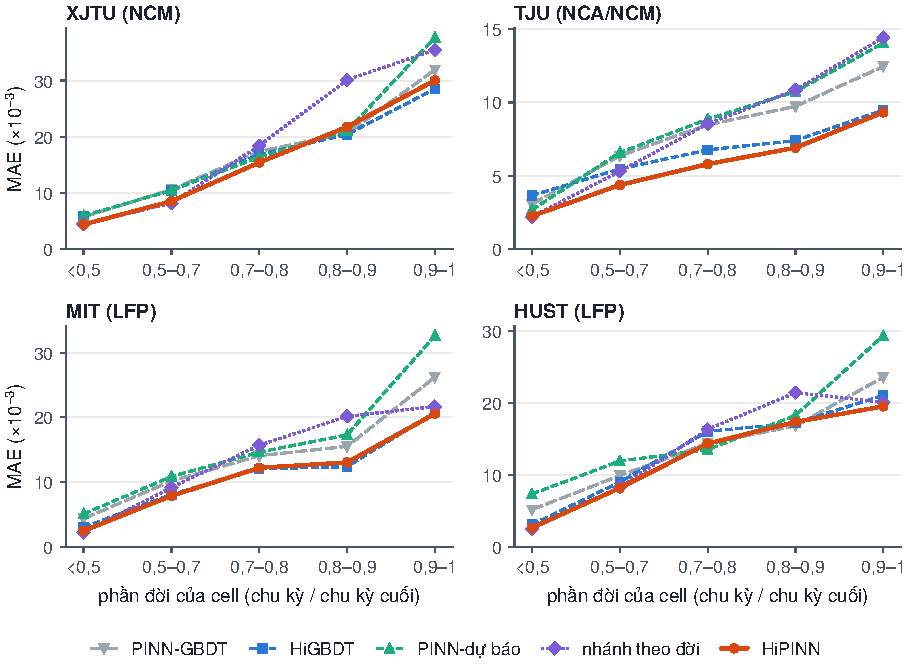
\includegraphics[width=\textwidth]{graphics/fig_e33_tail.pdf}
\caption[Sai số dự báo theo phần đời của cell]{MAE ($\times10^{-3}$) của SOH dự báo theo phần đời của chính cell (chu kỳ chia chu kỳ cuối ghi được), mọi cell huấn luyện, lịch sử đo, trung bình theo cell. Phần đời chỉ dùng để chia nhóm khi chấm, mô hình không biết nó.}\label{fig:e33tail}
\end{figure}

\Cref{fig:e33traj} minh hoạ dự báo cho một cell mỗi bộ. Ở mỗi tầm, HiPINN trùng với nhánh nằm giữa trong ba nhánh, nên đường của nó gãy khúc ở chỗ hai nhánh cắt nhau. Hình chỉ vẽ hai nhánh có đặc trưng lịch sử. Ở những đoạn HiPINN không trùng đường nào trong hai đường đó, nhánh nằm giữa là PINN-dự báo.

\begin{figure}[!htbp]\centering
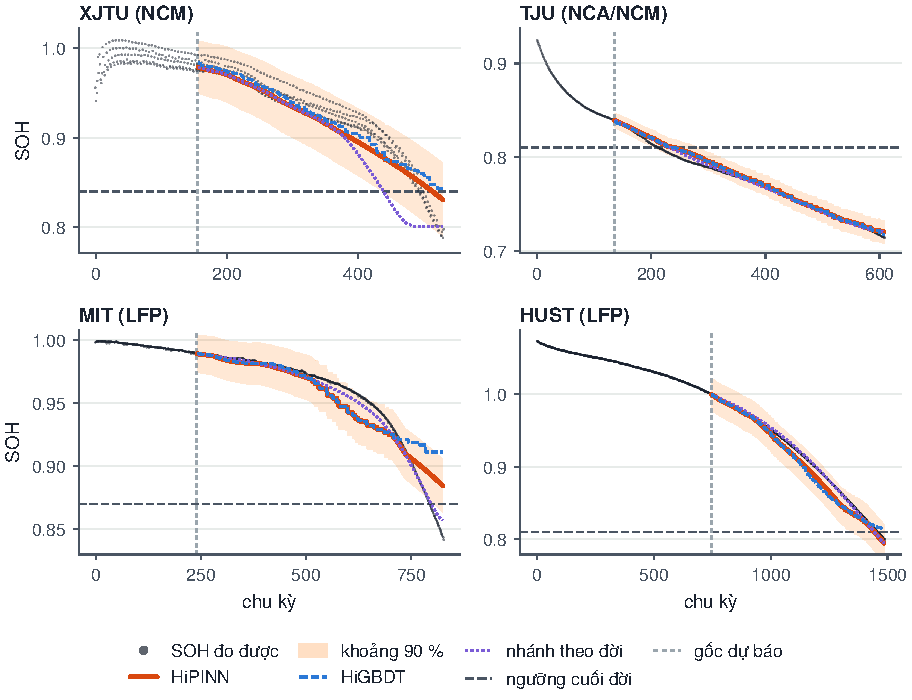
\includegraphics[width=\textwidth]{graphics/fig_e33_traj.pdf}
\caption[Dự báo của HiPINN so với SOH đo được]{Dự báo của HiPINN, HiGBDT và nhánh theo đời so với SOH đo được cho một cell kiểm tra mỗi bộ: mọi cell huấn luyện, lịch sử đo, lần lặp 0, gốc ở $0{,}4L$; trong các cell còn ít nhất $0{,}25L$ chu kỳ đo sau gốc, chọn cell có sai số của HiPINN ở trung vị. Khoảng 90\,\% tính bằng phương pháp conformal. PINN-dự báo, nhánh thứ ba của HiPINN, không vẽ để hình dễ đọc. Ở XJTU, cell được chọn thuộc nhóm R2.5, nhóm có chế độ xả thay đổi. Dung lượng đo của cell này lặp lại theo vòng 5 chu kỳ: chênh lệch trung bình giữa hai chu kỳ cách nhau 5 là 2{,}8 ($\times10^{-3}$), so với 8{,}3--12{,}5 ở các khoảng cách 1--4 chu kỳ. Vì vậy các điểm đo xếp thành 5 dải song song; đó là đặc điểm của dữ liệu, không phải nhiều cell vẽ chồng lên nhau.}\label{fig:e33traj}
\end{figure}

Có một điểm cần lưu ý khi đọc các kiểm định. Ở TJU, có 2 phép so mà kiểm định ghép cặp và MAE trung bình chỉ hai hướng khác nhau: phần lớn cell đi theo hướng của kiểm định, còn trung bình bị kéo bởi vài cell sai rất lớn. Bỏ 1--2 cell như vậy thì trung bình cũng đổi chiều. Cell gây chênh lệch lớn nhất là CY25-025\_1-\#1 của TJU: MAE của PINN-dự báo 241, của HiGBDT 42, của HiPINN 42 ($\times10^{-3}$).

Về RUL và khoảng dự báo, \Cref{tab:e33rul} cho MAE của RUL. Với mọi cell huấn luyện, RUL của HiPINN có MAE bằng 0{,}90--1{,}70 lần PINN-GBDT (thấp hơn có ý nghĩa thống kê trên TJU và MIT) và 0{,}34--0{,}80 lần HiGBDT (thấp hơn có ý nghĩa thống kê trên cả bốn bộ). Tỉ lệ RUL dự báo nằm trong $\pm 20\,\%$ RUL thực là 53--84\,\%. HiGBDT dự báo RUL dài hơn thực tế trên MIT và HUST (sai số có dấu trung bình MIT +201 và HUST +477 chu kỳ), cùng nguyên nhân với độ lệch dương ở phần cuối đời. Khoảng SOH 90\,\% của HiPINN phủ 89--93\,\% và khoảng RUL 90\,\% phủ 68--87\,\% tuỳ bộ, tức có bộ chưa đạt độ phủ danh nghĩa. Phân vị của khoảng chỉ tính trên vài cell hiệu chỉnh mỗi lượt.

\begin{table}[!htbp]\centering\small
\caption[MAE của RUL dự báo theo mô hình]{MAE của RUL (chu kỳ), trung bình qua các gốc ở 25, 50 và 75\,\% chu kỳ cuối đời thật và qua 3 lần lặp; in đậm là thấp nhất mỗi hàng. Cột RUL thực là RUL thật trung bình, để đối chiếu cỡ sai số. Hai cột cuối là của HiPINN: tỉ lệ RUL dự báo nằm trong $\pm20\,\%$ RUL thực (cao hơn là tốt hơn) và độ phủ của khoảng RUL 90\,\% (tốt nhất là gần 90\,\%). $^{*}$/$^{\dagger}$: RUL của HiPINN tốt hơn/kém hơn có ý nghĩa thống kê so với PINN-GBDT (Wilcoxon ghép cặp theo cell, hiệu chỉnh Holm qua bốn bộ, $p<0{,}05$); không có dấu: khác biệt không có ý nghĩa thống kê.}\label{tab:e33rul}
\begin{adjustbox}{max width=\textwidth}\begin{tabular}{lrrrrrrrrrrr}\toprule
 & & \multicolumn{8}{c}{MAE của RUL (chu kỳ) $\downarrow$} & \multicolumn{2}{c}{HiPINN} \\\cmidrule(lr){3-10}\cmidrule(lr){11-12}
Bộ & \begin{tabular}[b]{@{}r@{}}RUL\\thực\end{tabular} & \begin{tabular}[b]{@{}r@{}}GBDT\\theo tầm\end{tabular} & \begin{tabular}[b]{@{}r@{}}PINN-\\dự báo\end{tabular} & \begin{tabular}[b]{@{}r@{}}PINN-\\GBDT\end{tabular} & \begin{tabular}[b]{@{}r@{}}\\HiGBDT\end{tabular} & \begin{tabular}[b]{@{}r@{}}PINN có\\lịch sử\end{tabular} & \begin{tabular}[b]{@{}r@{}}Theo\\đời\end{tabular} & \begin{tabular}[b]{@{}r@{}}\\HiPINN-w\end{tabular} & \begin{tabular}[b]{@{}r@{}}\\HiPINN\end{tabular} & \begin{tabular}[b]{@{}r@{}}Trong\\$\pm20\,\%$ $\uparrow$\end{tabular} & \begin{tabular}[b]{@{}r@{}}Độ phủ\\(90\,\%)\end{tabular} \\\midrule
\multicolumn{12}{@{}l}{\textit{30\,\% nhãn}} \\
XJTU & 231 & 98 & 84 & 77 & 139 & 75 & \textbf{67} & 72 & 74\phantom{$^{*}$} & 42\,\% & 77\,\% \\
TJU & 131 & 19 & 18 & 16 & 19 & 18 & 18 & \textbf{15} & 15\phantom{$^{*}$} & 74\,\% & 83\,\% \\
MIT & 344 & 139 & 124 & 112 & 369 & 108 & \textbf{83} & 164 & 115\phantom{$^{*}$} & 49\,\% & 73\,\% \\
HUST & 923 & 210 & 134 & 140 & 598 & \textbf{129} & 832 & 291 & 211\phantom{$^{*}$} & 77\,\% & 77\,\% \\
\addlinespace[3pt]
\multicolumn{12}{@{}l}{\textit{mọi cell huấn luyện}} \\
XJTU & 231 & 110 & 70 & 66 & 96 & 64 & \textbf{53} & 59 & 61\phantom{$^{*}$} & 53\,\% & 75\,\% \\
TJU & 131 & 17 & 14 & 14 & 16 & 13 & 14 & 12 & \textbf{12}$^{*}$ & 82\,\% & 87\,\% \\
MIT & 344 & 134 & 113 & 108 & 229 & 103 & \textbf{76} & 126 & 97$^{*}$ & 53\,\% & 68\,\% \\
HUST & 923 & 198 & 94 & 103 & 512 & \textbf{92} & 676 & 137 & 176\phantom{$^{*}$} & 84\,\% & 79\,\% \\
\bottomrule\end{tabular}\end{adjustbox}\end{table}

Để gợi ý một mô hình cho lần dùng sau, ba mô hình HiPINN, HiGBDT và PINN-GBDT được so theo cùng một quy tắc, áp riêng cho từng ngân sách nhãn: mô hình được chọn phải có MAE thấp hơn từng mô hình còn lại trên ít nhất ba bộ và không kém có ý nghĩa thống kê trên bộ nào. Quy tắc này và dạng trung vị của HiPINN đều được đặt sau khi đã có kết quả trên tập kiểm tra, nên lựa chọn dưới đây chỉ là gợi ý, chưa được kiểm chứng trên dữ liệu mới. Với SOH, quy tắc chọn HiPINN ở cả hai ngân sách. Với RUL ở 30\,\% nhãn, không mô hình nào thoả quy tắc: MAE RUL của HiPINN chỉ thấp hơn PINN-GBDT ở 2/4 bộ. Với RUL khi học trên mọi cell huấn luyện, quy tắc chọn HiPINN. Riêng trên HUST, MAE RUL của HiPINN cao hơn PINN-GBDT ở cả hai ngân sách (176 so với 103 chu kỳ khi học trên mọi cell huấn luyện, gấp 1{,}70 lần). Khác biệt này không có ý nghĩa thống kê vì HiPINN vẫn tốt hơn ở 44/74 cell, còn MAE trung bình bị vài cell sai rất lớn kéo lên: HiGBDT và nhánh theo đời cùng dự báo RUL dài hơn thực tế ở các cell đó, nên trung vị đi theo chúng. Với các cell giống HUST, mô hình không dùng lịch sử như PINN-GBDT cho RUL an toàn hơn.
